\documentclass[UTF8,11pt,a4paper]{ctexart}

\usepackage[a4paper,margin=2.05cm]{geometry}
\usepackage{amsmath,amssymb}
\usepackage{array}
\usepackage{booktabs}
\usepackage{caption}
\usepackage{enumitem}
\usepackage{float}
\usepackage{fontspec}
\usepackage{graphicx}
\usepackage{hyperref}
\usepackage{longtable}
\usepackage{makecell}
\usepackage{microtype}
\usepackage{multirow}
\usepackage{subcaption}
\usepackage{tabularx}
\usepackage{threeparttable}
\usepackage{tikz}
\usepackage{tocloft}
\usepackage{xcolor}
\usepackage{setspace}
\usepackage[ruled,vlined,linesnumbered]{algorithm2e}
\usepackage[backend=biber,style=numeric,sorting=none,maxbibnames=99]{biblatex}

\usetikzlibrary{arrows.meta,calc,fit,positioning,shapes.geometric}
\graphicspath{{figures/}}
\addbibresource{references.bib}

\setmainfont{Times New Roman}
\setsansfont{Helvetica Neue}
\setmonofont{Menlo}
\setCJKmainfont{Songti SC}
\setCJKsansfont{PingFang SC}
\setCJKmonofont{PingFang SC}

\definecolor{Ink}{HTML}{1F2937}
\definecolor{Muted}{HTML}{64748B}
\definecolor{Line}{HTML}{CBD5E1}
\definecolor{SoftBlue}{HTML}{E8F1F8}
\definecolor{SoftAmber}{HTML}{FFF1D8}
\definecolor{SoftGreen}{HTML}{E9F4EF}
\definecolor{SoftRed}{HTML}{FBEAE8}
\definecolor{Blue}{HTML}{3973AC}
\definecolor{Amber}{HTML}{D0902F}
\definecolor{Green}{HTML}{4F8A70}
\definecolor{Red}{HTML}{B44C43}

\hypersetup{
  colorlinks=true,
  linkcolor=Blue,
  citecolor=Blue,
  urlcolor=Blue,
  pdftitle={语义不变性不等于表示不变性：真实中文噪声下结构化抽取的模式条件规范投影},
  pdfauthor={高展沛}
}

\captionsetup{font=small,labelfont=bf}
\setstretch{1.06}
\setlength{\parindent}{2em}
\setlength{\parskip}{0.12em}
\setlist[itemize]{leftmargin=2em,itemsep=0.12em,topsep=0.2em}
\setlist[enumerate]{leftmargin=2.2em,itemsep=0.12em,topsep=0.2em}
\emergencystretch=2em
\renewcommand{\arraystretch}{1.12}
\renewcommand{\contentsname}{目录}
\setlength{\cftbeforetoctitleskip}{0.1cm}
\setlength{\cftaftertoctitleskip}{1.1em}
\renewcommand{\cfttoctitlefont}{\Huge\bfseries}
\renewcommand{\cftsecfont}{\fontsize{16bp}{19bp}\selectfont\bfseries}
\renewcommand{\cftsecpagefont}{\fontsize{16bp}{19bp}\selectfont\bfseries}
\renewcommand{\cftsecleader}{\cftdotfill{\cftsecdotsep}}
\renewcommand{\cftsecdotsep}{\cftdotsep}
\setlength{\cftsecindent}{0em}
\setlength{\cftsecnumwidth}{2.2em}
\setlength{\cftbeforesecskip}{1.50em}
\renewcommand{\cftsubsecfont}{\fontsize{13.8bp}{17bp}\selectfont}
\renewcommand{\cftsubsecpagefont}{\fontsize{13.8bp}{17bp}\selectfont}
\renewcommand{\cftsubsecleader}{\cftdotfill{\cftsubsecdotsep}}
\renewcommand{\cftsubsecdotsep}{\cftdotsep}
\setlength{\cftsubsecindent}{2.2em}
\setlength{\cftsubsecnumwidth}{3.0em}
\setlength{\cftbeforesubsecskip}{0.24em}
\SetAlgorithmName{算法}{算法}{算法列表}
\SetKwInput{KwIn}{输入}
\SetKwInput{KwOut}{输出}
\SetKw{KwRet}{返回}
\DontPrintSemicolon
\newcolumntype{Y}{>{\raggedright\arraybackslash}X}
\newcommand{\method}{SCCP}
\newcommand{\dataset}{CanoInvar-ZH}
\newcommand{\gap}{\mathrm{Gap}}
\newcommand{\pp}{pp}
\newcommand{\papertitlecn}{语义不变性不等于表示不变性：\\真实中文噪声下结构化抽取的模式条件规范投影}
\newcommand{\papertitleen}{Semantic Invariance Is Not Representational Invariance:\\Schema-Conditioned Canonical Projection for Robust Chinese Structured Extraction}
\newcommand{\paperauthor}{高展沛}
\newcommand{\paperid}{2023212036}
\newcommand{\paperdate}{2026年6月9日}

\begin{document}
\hypersetup{pageanchor=false}
\pagenumbering{gobble}

\begin{titlepage}
  \centering
  \vspace*{2.8cm}
  {\LARGE\bfseries \papertitlecn\par}
  \vspace{0.55cm}
  {\large \papertitleen\par}
  \vspace{3.0cm}
  {\large \paperauthor\par}
  \vspace{0.25cm}
  {\large \paperid\par}
  \vfill
  {\large \paperdate\par}
\end{titlepage}

\clearpage
\begin{center}
  {\Large\bfseries 摘要}
\end{center}
\vspace{0.55cm}
\begin{center}
\begin{minipage}{0.88\linewidth}
\setstretch{1.12}
真实中文输入常包含简繁混写、全半角混排和 OCR 易混字符。对人类而言，这些扰动通常不改变事实语义；对结构化抽取系统而言，它们却可能使 company、date 和 amount 等字段落入不同的表面字符串，从而触发精确匹配失败。本文提出一个机制性解释：\textbf{语义不变性不等于表示不变性}。现有鲁棒提示主要试图修复模型的理解阶段，但错误根因往往出现在语义表示投影到模式约束字段空间的最后一步，即 canonicalization gap。基于这一观察，本文提出模式条件规范投影（Schema-Conditioned Canonical Projection, \method{}）：先根据字段模式路由到字符、数值和实体规范算子，再生成规范候选并通过源文本一致性与格式约束选择最终字段。在 \dataset{} 中文规范不变性评测集上，本文评估五个前沿模型和四类提示下的成对抽取表现。实验显示，普通提示下简繁变体和 OCR 易混字符的不变性差距分别达到 55.23\pp{} 和 65.26\pp{}，且不同提示之间几乎没有实质缓解；在独立校准注册表构建的严格设置下，\method{} 将二者降至 0.00\pp{} 和 14.36\pp{}，并消除原有的跨模型显著性证据。进一步的 seen/unseen 分析表明，已登录实体上的 OCR 差距仅为 3.44\pp{}，未登录实体仍为 35.89\pp{}，说明规范投影有效但受实体覆盖率约束。本文由此把“噪声鲁棒性”重新定位为结构化抽取中的规范投影问题，并给出可复现、可追踪、可消融的解决路径。

\vspace{0.75cm}
\noindent\textbf{关键词：}结构化抽取；中文噪声；实体规范化；约束解码；大语言模型鲁棒性
\end{minipage}
\end{center}

\clearpage
\thispagestyle{empty}
\tableofcontents

\clearpage
\hypersetup{pageanchor=true}
\pagenumbering{arabic}
\setcounter{page}{1}

\section{引言}

结构化抽取系统把自然语言文本映射为可计算字段。这个过程看似只是让模型输出一个结构化对象，实际却包含两个不同层面的要求：模型需要理解文本中的事实，也需要把事实投影到下游系统接受的规范表示。第二个要求在干净英文基准中常被忽略，但在真实中文场景中变得非常尖锐。企业公告、客服记录、聊天消息和表单 OCR 往往混入“藍海數據”“Z026”“IS00万元”这类表面变体。人类读者很容易恢复其含义；结构化接口却可能把“藍海數據A1”和“蓝海数据A1”视为不同实体，把“IS00万元”和“1500万元”视为不同金额。

这类错误容易被误诊为“模型没有理解脏数据”。本文的核心观点恰恰相反：许多失败并不发生在事实理解本身，而发生在理解之后的\textbf{规范投影}阶段。若一个扰动 $T$ 保持事实语义不变，理想抽取器应满足
\[
  \pi_S(f(x))=\pi_S(f(T(x))),
\]
其中 $f$ 是模型生成的表面字段，$\pi_S$ 是由字段模式 $S$ 决定的规范投影。没有 $\pi_S$ 时，模型即使识别了同一事实，也可能复制扰动后的表面字符串，导致结构化输出失配。这就是本文称为 canonicalization gap 的根因。

图~\ref{fig:gap} 给出了这一机制的简单示意。传统提示增强主要在“输入理解”或“输出格式”处施力：提醒模型注意噪声、要求 JSON、给出少样例。但如果任务真正要求的是落入 company、date、amount 各自的规范空间，仅靠更长提示无法稳定完成字段级等价类收束。在五个模型、四类提示上观察到相同模式：P1--P4 的提示差异几乎不能改变强噪声机制的不变性差距，简繁变体始终约 55\pp{}，OCR 易混字符始终约 60--70\pp{}。

\begin{figure}[H]
\centering
\begin{tikzpicture}[
  x=1cm,y=1cm,
  font=\small,
  input/.style={draw=Blue, fill=SoftBlue, rounded corners=2pt, align=center, minimum width=2.35cm, minimum height=0.86cm},
  fact/.style={draw=Line, fill=gray!8, rounded corners=2pt, align=center, minimum width=2.35cm, minimum height=0.98cm},
  surface/.style={draw=Red, fill=SoftRed, rounded corners=2pt, align=center, minimum width=2.55cm, minimum height=0.86cm},
  proj/.style={draw=Amber, fill=SoftAmber, rounded corners=2pt, align=center, minimum width=2.25cm, minimum height=0.98cm},
  canon/.style={draw=Green, fill=SoftGreen, rounded corners=2pt, align=center, minimum width=2.35cm, minimum height=0.86cm},
  note/.style={draw=Red, fill=SoftRed, rounded corners=2pt, align=center, text width=11.8cm, minimum height=0.74cm},
  phase/.style={font=\small\bfseries, text=Muted},
  arr/.style={-{Latex[length=2.0mm]}, line width=0.75pt, draw=Ink}
]
  \node[phase] at (1.25,2.15) {输入扰动};
  \node[phase] at (4.25,2.15) {语义合流};
  \node[phase] at (7.45,2.15) {表示分叉};
  \node[phase] at (12.35,2.15) {规范合流};

  \node[input] (x1) at (1.25,1.15) {原始输入 $x$\\蓝海数据A1};
  \node[input] (x2) at (1.25,-1.15) {扰动输入 $T(x)$\\藍海數據A1};
  \node[fact] (fact) at (4.25,0) {同一事实\\$z(x)=z(T(x))$};
  \node[surface] (s1) at (7.45,1.15) {表面字段一\\蓝海数据A1};
  \node[surface] (s2) at (7.45,-1.15) {表面字段二\\藍海數據A1};
  \node[proj] (proj) at (10.65,0) {模式条件\\投影 $\pi_S$};
  \node[canon] (canon) at (13.55,0) {规范字段\\蓝海数据A1};
  \node[note, text=Red] at (7.45,-2.65) {缺少模式条件投影时，语义等价的输入会在表面字符串空间分叉；结构化抽取需要把它们重新投影到同一规范字段。};

  \draw[arr] (x1.east) -- (fact.west);
  \draw[arr] (x2.east) -- (fact.west);
  \draw[arr] (fact.east) -- (s1.west);
  \draw[arr] (fact.east) -- (s2.west);
  \draw[arr] (s1.east) -- (proj.west);
  \draw[arr] (s2.east) -- (proj.west);
  \draw[arr] (proj.east) -- (canon.west);
\end{tikzpicture}
\caption{Canonicalization gap 的根因：扰动保持事实语义不变，但模型输出仍处于表面字符串空间；结构化抽取要求字段落入由模式定义的规范空间。}
\label{fig:gap}
\end{figure}

针对这一根因，本文提出 \method{}。它不是新的大模型，也不是一次性提示，而是一类可组合的规范投影策略：由字段模式决定调用哪些规范算子，分别处理脚本/全半角、日期金额数值和实体候选投影。这个设计把“鲁棒性”从泛泛的输入噪声问题，收窄为可检验的字段投影问题。本文贡献如下：

\begin{itemize}
  \item 提出 canonicalization gap 作为真实中文噪声下结构化抽取失败的机制性解释，区分语义理解错误与规范表示错误。
  \item 构建 \dataset{} 成对评测协议，在五模型四提示设置下显示 prompt-only 鲁棒提示不能稳定修复投影阶段失效。
  \item 提出 \method{}，将字符、数值与实体规范化抽象为 schema-conditioned canonical projection，并在严格无泄漏设置下显著缩小不变性差距。
  \item 通过 seen/unseen 分析指出方法边界：闭集实体上投影几乎消解 OCR 断裂，未登录实体则暴露开放世界规范化困难。
\end{itemize}



\begin{figure}[H]
\centering
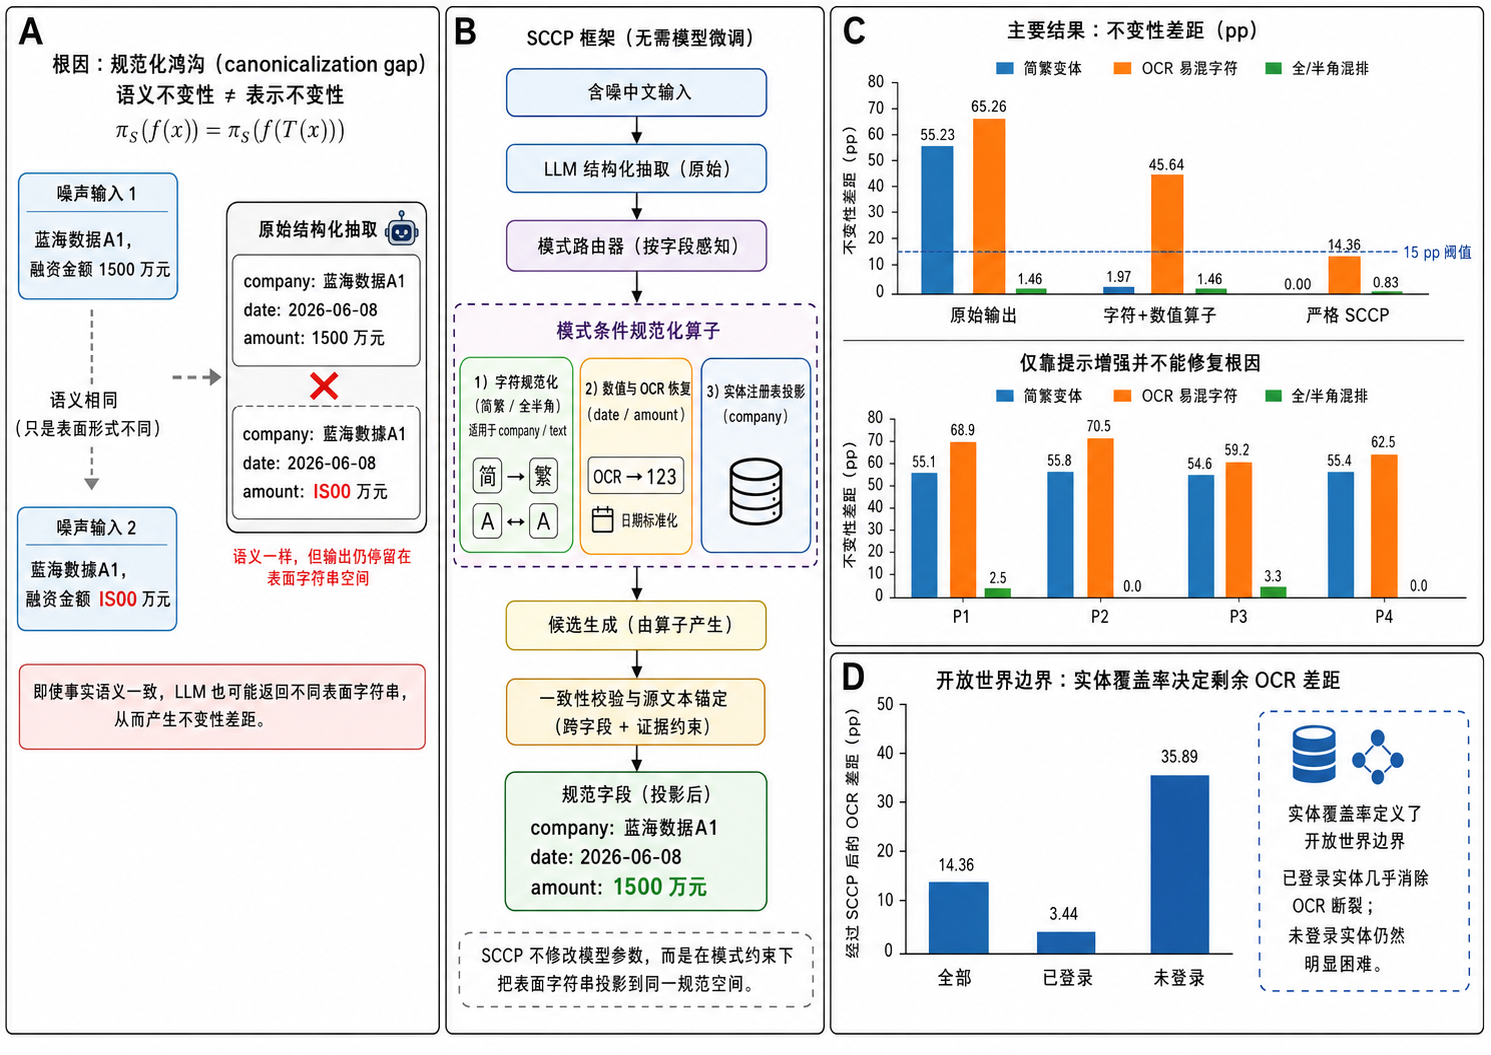
\includegraphics[width=0.98\linewidth]{main.png}
\caption{总结本文从根因、方法到实验证据的整体链条。A：canonicalization gap 的机制性根因；B：\method{} 的模式条件规范投影框架；C：严格设置下的主结果与 prompt-only 失效；D：实体覆盖率揭示的开放世界边界。}
\label{fig:paper_main}
\end{figure}

\section{相关工作}

\paragraph{噪声鲁棒性与行为测试。}
输入扰动会影响神经语言模型的稳定性，相关研究覆盖字符替换、拼写噪声、指令噪声和多语言真实噪声等设定 \cite{moradi-samwald-2021-evaluating,wang-etal-2024-resilience,aliakbarzadeh-etal-2025-exploring,michail-etal-2025-cheap}。CheckList 强调通过行为测试定位具体能力缺陷，而不是只报告总体准确率 \cite{ribeiro-etal-2020-checklist}。本文沿用成对行为测试思想，但关注结构化抽取中更细的字段规范不变性：扰动不改变事实时，规范字段是否保持一致。

\paragraph{中文变体与 OCR 规范化。}
简繁转换和 OCR 纠错本身有长期研究。上下文感知简繁转换说明脚本变体并不等价于简单字符替换，仍需要显式规范化机制 \cite{li-etal-2024-unsupervised}。OCR 噪声鲁棒表示研究表明，视觉相近字符会系统影响多语言模型表示 \cite{michail-etal-2025-cheap}。本文不把这两类噪声视为孤立预处理问题，而是研究它们如何在 company、date、amount 等字段上被结构化接口放大。

\paragraph{结构化生成与约束解码。}
统一结构生成将信息抽取表述为可生成的结构对象 \cite{lu-etal-2022-unified}；语法约束解码和 guided generation 进一步表明，形式约束可以在不微调模型的情况下提高结构输出可靠性 \cite{geng-etal-2023-grammar,willard-louf-2023-guided}。这些工作主要保证输出形状或语法合法性。本文处理的是另一层约束：字段值即使语法合法，也必须落入 schema 所规定的规范等价类。

\paragraph{实体规范化与实体检索。}
实体规范化将噪声 mention 映射到标准实体，常见于生物医学和知识库任务 \cite{ji-etal-2020-bert-normalization}；GENRE 等自回归实体检索方法则展示了通过生成实体名称完成开放实体匹配的可能性 \cite{de-cao-etal-2021-autoregressive}。本文借鉴“候选实体空间”思想，但场景不是通用实体链接，而是结构化抽取输出后的字段级规范投影。

\paragraph{组合式推断与透明评测。}
ReAct 和 Toolformer 展示了语言模型与外部行动或工具交互的价值 \cite{yao-etal-2023-react,schick-etal-2023-toolformer}。HELM 则从场景和指标覆盖角度强调透明评测 \cite{liang-etal-2022-helm}。本文借鉴这两类思想，但将其收束为确定性、可审计的组合式规范策略：所有字段决策都来自固定投影算子与显式验证条件，而不是开放式探索过程。

\section{问题形式化}

设输入文本为 $x$，扰动函数 $T$ 保持事实语义不变，即 $z(x)=z(T(x))$。结构化抽取模型产生字段字典
\[
  y=f_\theta(x)=\{y_c,y_d,y_a\},
\]
其中 $c,d,a$ 分别表示 company、date 和 amount。传统评测直接比较 $y$ 与金标准 $g$ 的表面字符串。本文认为，更合理的结构化目标应先定义字段规范空间 $\mathcal{C}_S$，并通过模式条件投影 $\pi_S$ 得到
\[
  \hat{y}=\pi_S(y,x,\mathcal{R}),
\]
其中 $\mathcal{R}$ 是可选的实体注册表或规范候选集。系统失败可分为两类：若模型没有抽取到正确事实，则 $f_\theta$ 已经失败；若事实正确但字段没有投影到规范表示，则失败位于 $\pi_S$ 缺失或不完备。

用不变性差距度量扰动造成的配对错误增量：
\[
  \gap(m,p,t)=100\cdot
  \bigl(\Pr[e(T(x))=1]-\Pr[e(x)=1]\bigr),
\]
其中 $m,p,t$ 分别为模型、提示和扰动类型，$e(\cdot)$ 表示字段级错误事件。若某个模型-提示-扰动单元的差距超过 15\pp{} 且 McNemar 精确检验显著，则记为单元级失效；若同一模型多提示失效，再扩展为模型级证据。这个层级统计用于判断问题是否跨提示、跨模型稳定存在。

在有实体注册表的情况下，\method{} 的理论预期可写为
\[
  \gap_{\method{}}(t)
  \approx \rho\,\gap_{\mathrm{seen}}(t)+(1-\rho)\,\gap_{\mathrm{unseen}}(t)+\epsilon_{\mathrm{route}},
\]
其中 $\rho$ 是测试实体被注册表覆盖的比例，$\epsilon_{\mathrm{route}}$ 是字段路由和算子选择误差。这个分解给出两个可检验预测：已登录实体应显著受益于实体投影；未登录实体仍会保留较大开放世界误差。

\section{方法：模式条件规范投影}

\subsection{总体框架}

\method{} 的目标是在模型原始输出与下游规范空间之间加入一个显式、可追踪的投影层。图~\ref{fig:sccp_arch} 展示了方法结构。首先，结构化候选生成器输出 company、date、amount 的表面值；其次，模式路由器根据字段类型选择规范算子；然后，字符、数值和实体算子生成候选集合；最后，一致性验证器根据格式合法性、源文本锚定和注册表匹配选择最终字段。每个投影决策记录字段、候选、算子和触发条件，便于后续审计。

\begin{figure}[H]
\centering
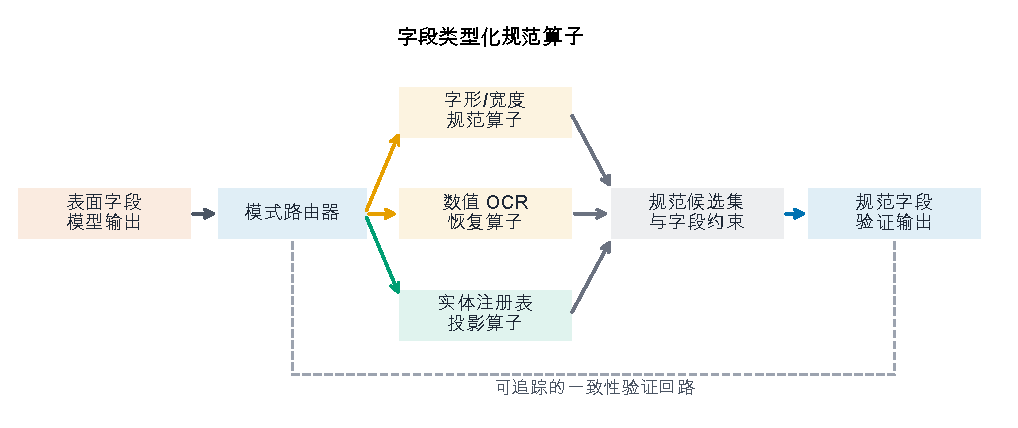
\includegraphics[width=\linewidth]{sccp_architecture}
\caption{\method{} 方法架构。方法不改变模型参数，而是在字段模式约束下将表面候选投影到规范空间。}
\label{fig:sccp_arch}
\end{figure}

这个推断图反应本研究关注可复现的机制验证：若一个系统同时修改输入、提示、后处理和评分，却不记录每个投影决策，就无法回答“究竟是哪一环修复了问题”。因此，本文将外部知识、局部规则和评测反馈抽象为可组合算子与可追踪推断策略。

\subsection{字段类型化算子}

\paragraph{字符算子。}
字符算子负责简繁统一与全半角统一。它适用于所有字段，但对 company 的帮助最明显。该算子只执行确定性映射，不使用测试标签。

\paragraph{数值算子。}
date 与 amount 具有强格式约束。数值算子将 OCR 易混字符映射回数字，例如 $Z\rightarrow2$、$I\rightarrow1$、$S\rightarrow5$，再调用日期和金额格式化规则。由于字段模式明确，数值算子不会把 company 中的英文后缀任意删除。

\paragraph{实体算子。}
company 是实体字段，不能只靠字符替换。实体算子将模型输出、源文本和候选实体统一到 compact key 空间，比较脚本等价、OCR 等价和源文本锚定条件。若候选满足高置信条件，则输出注册表中的规范实体。

\subsection{投影策略}

给定模型输出 $y$、源文本 $x$ 和注册表 $\mathcal{R}$，\method{} 对每个字段独立生成候选，再按字段约束选择最终值。算法~\ref{alg:sccp_projection} 给出字段级投影过程。

\begin{algorithm}[H]
\small
\caption{\method{} 的字段级规范投影过程}
\label{alg:sccp_projection}
\KwIn{模型输出 $y$、源文本 $x$、字段模式 $S$、实体注册表 $\mathcal{R}$}
\KwOut{规范字段 $\hat{y}$ 与投影动作记录 $a$}
解析 $y$，获得 company、date、amount 的表面候选\;
\ForEach{$k \in \{\mathrm{company}, \mathrm{date}, \mathrm{amount}\}$}{
  根据字段模式 $S_k$ 选择字符、数值或实体规范算子\;
  \eIf{$k \in \{\mathrm{date}, \mathrm{amount}\}$}{
    执行 OCR 数字恢复，并按日期或金额格式生成候选\;
  }{
    执行简繁与全半角统一，计算实体 OCR 等价 key\;
    若候选与 $\mathcal{R}$ 中实体满足脚本等价、OCR 等价或源文本锚定条件，则投影为注册表规范实体\;
  }
  根据格式合法性、源文本一致性和注册表匹配选择 $\hat{y}_k$\;
  记录字段、候选、触发算子和选择原因到 $a$\;
}
若无高置信候选，则保留保守规范化后的原字段\;
\KwRet{$\hat{y}, a$}\;
\end{algorithm}

\section{实验设置}

\subsection{数据与任务}

\dataset{} 包含真实中文应用中常见的六类来源：公告、客服对话、社交媒体、邮件、即时聊天和表单 OCR。主评测集包含 96 个 extraction 成对样本、192 条输入；每个 pair 包含 control 与 perturbed 两个版本，二者共享同一规范金标准。三类扰动分别为简繁变体、全半角混排和 OCR 易混字符。字段分布刻意不均衡：简繁主要压力在 company，OCR 同时压力在 company、date 与 amount，全半角作为弱对照。

模型集合包括 GPT、Gemini、DeepSeek、GLM 和 Qwen 系列的五个代表模型；提示集合包括直接抽取、格式强化、少样例和鲁棒提示四类。所有主结果均基于同一批离线模型响应重评分，因此不同投影策略之间没有新模型调用随机性。

\subsection{严格注册表}

为避免测试标签泄漏，严格 \method{} 使用独立校准集构建实体注册表。校准注册表包含 12 个规范实体；主评测集包含 18 个实体，其中 12 个已登录、6 个未登录。这个设置模拟真实系统中“历史主数据覆盖部分实体”的闭集/开放世界混合条件。另外报告 oracle 上界，即使用主评测集实体集合构建注册表，说明覆盖充分时的理论上限。
\subsection{比较条件}

实验比较四个条件。第一，模型原始输出，即无规范投影。第二，字符与数值算子，仅执行简繁、全半角和 date/amount OCR 数字恢复。第三，严格 \method{}，在独立注册表上增加 company 实体投影。第四，oracle \method{}，使用测试集实体集合作为上界。

主指标为不变性差距 $\gap$。同时报告旧层级显著性证据：单元级差距阈值为 15\pp{}，并要求 McNemar 精确检验显著；若一个模型在多个提示下失效，则形成模型级证据。本文用该层级证据判断问题是否“跨提示、跨模型”稳定存在。

\section{结果}

\subsection{提示增强并未解决根因}

图~\ref{fig:prompt_heatmap} 显示，不同提示模板对强扰动几乎没有根本性影响。简繁变体在 P1--P4 下的不变性差距分别为 55.1、55.8、54.6 和 55.4\pp{}；OCR 易混字符分别为 68.9、70.5、59.2 和 62.5\pp{}。少样例或鲁棒提示可以在个别单元上略有波动，但没有改变“语义等价输入投影为不同规范字段”的核心失败。

\begin{figure}[H]
\centering
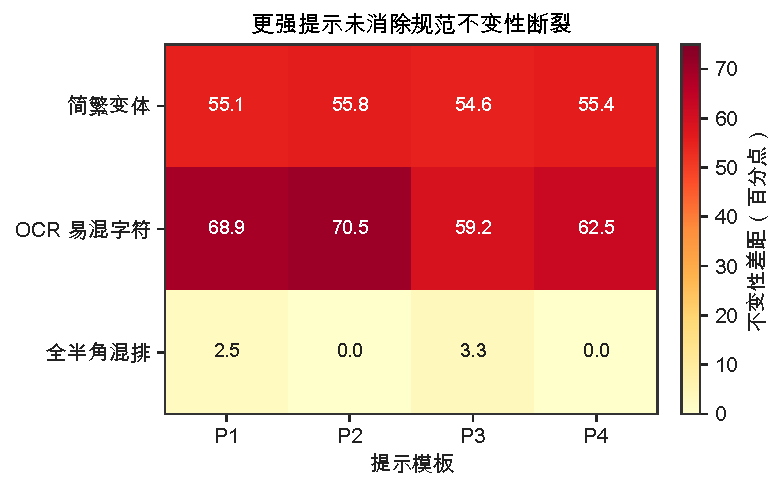
\includegraphics[width=0.93\linewidth]{sccp_prompt_invariance}
\caption{五模型均值下的提示增强效果。强扰动机制在四类提示下均保持高不变性差距，说明错误不只是提示说明不足。}
\label{fig:prompt_heatmap}
\end{figure}

这个观察支持本文的机制假设：如果失败主要发生在最终规范投影阶段，那么改变自然语言提示并不能稳定弥合 canonicalization gap。提示可以要求模型“注意噪声”，但不能保证 company 落入实体规范空间，也不能保证 OCR 字符在数值槽位中被系统恢复。

\subsection{严格 SCCP 缩小不变性差距}

表~\ref{tab:main_result} 和图~\ref{fig:main_result} 给出主结果。模型原始输出下，简繁变体与 OCR 易混字符分别产生 55.23\pp{} 和 65.26\pp{} 的不变性差距，并在五个模型上都形成稳定证据。字符与数值算子将简繁变体降至 1.97\pp{}，但 OCR 仍为 45.64\pp{}，说明 company 槽位需要实体投影。严格 \method{} 进一步将 OCR 降至 14.36\pp{}，低于 15\pp{} 阈值，且不再有任何模型满足跨提示证据。

\begin{table}[H]
\centering
\small
\caption{主评测集上的不变性差距（百分点）。}
\label{tab:main_result}
\begin{tabular}{lccc}
\toprule
条件 & 简繁变体 & OCR 易混字符 & 全半角混排 \\
\midrule
模型原始输出 & 55.23 & 65.26 & 1.46 \\
字符与数值算子 & 1.97 & 45.64 & 1.46 \\
\method{}（严格） & 0.00 & 14.36 & 0.83 \\
\method{}（oracle 上界） & 0.00 & 2.92 & 0.00 \\
\bottomrule
\end{tabular}
\end{table}

\begin{figure}[H]
\centering
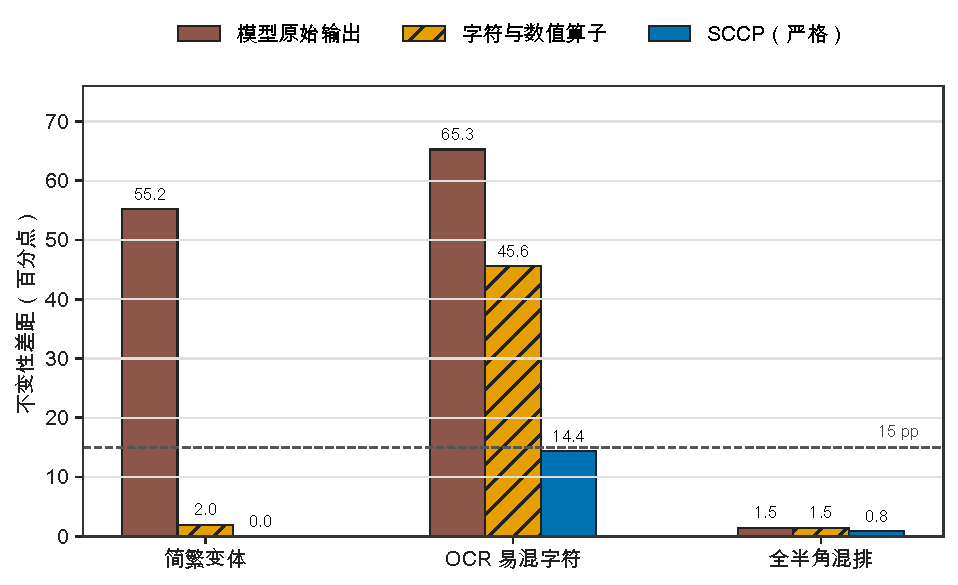
\includegraphics[width=0.96\linewidth]{sccp_main_results}
\caption{\method{} 主结果。严格设置不使用测试实体标签，仍显著缩小两类主扰动的不变性差距。}
\label{fig:main_result}
\end{figure}

这些结果给出清晰的因果链条。简繁问题主要是脚本变体保留，因此字符算子足以修复大部分失败；OCR 问题同时污染数值字段和公司实体，单纯数值恢复无法处理“B8/8B/A1/AI”一类实体编号混淆。加入 schema-conditioned entity projection 后，错误显著下降。

\subsection{实体覆盖率揭示开放世界边界}

图~\ref{fig:coverage} 展示了 seen/unseen 分析。严格 \method{} 在已登录实体上几乎消除投影断裂：OCR 易混字符仅剩 3.44\pp{}。但在未登录实体上，OCR 差距仍为 35.89\pp{}。这与形式化分解一致：当 $\rho$ 较低或目标实体未出现在注册表中，实体算子无法可靠判断表面字符串应投影到哪个规范实体。

\begin{figure}[H]
\centering
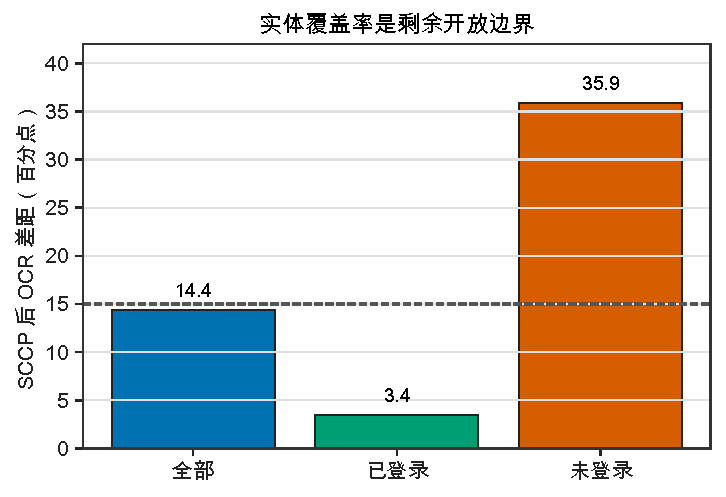
\includegraphics[width=0.92\linewidth]{sccp_coverage_boundary}
\caption{实体覆盖率决定 \method{} 的开放世界边界。已登录实体几乎消除 OCR 断裂，未登录实体仍需要更强候选发现或开放实体链接。}
\label{fig:coverage}
\end{figure}

这个结果使本文的结论更加克制也更有解释力。\method{} 并不是“万能后处理器”，而是把失败从混乱的字符串错误拆解为两个可操作部分：已覆盖实体的规范投影，以及未覆盖实体的开放世界候选发现。前者可以用确定性注册表显著缓解；后者需要实体发现、检索或训练增强。

\subsection{在线可行性小片}

在可用平台模型上，额外完成了一个在线切片：使用 GLM-4.7 对 4 条样本、2 个提示进行普通输入、预处理输入和完整 \method{} 三种条件测试。普通输入得到 4/8 正确；预处理输入和完整 \method{} 均为 8/8 正确。
\section{案例分析}

\paragraph{简繁变体：理解正确但表示漂移。}
在一个简繁样例中，扰动输入包含“藍海數據A1”。模型输出 company 为“藍海數据A1”，date 与 amount 均正确。该错误不是融资事实理解失败，而是表面脚本被复制到 company 字段。字符算子将其投影为“蓝海数据A1”后，配对不变性恢复。

\paragraph{金额 OCR：强格式字段适合确定性恢复。}
在金额样例中，输入和模型输出都保留“IS00万元”。amount 字段具有明确数字模式，因此数值算子可将 $I$ 恢复为 1、$S$ 恢复为 5，得到“1500万元”。这说明 date/amount 的失败主要是格式槽位中的 OCR 字符污染。

\paragraph{实体 OCR：必须引入规范实体空间。}
在 company 样例中，模型输出“华澄资讯8B”，规范实体为“华澄资讯B8”。若只做字符替换，8B 可能被错误改写为 88；若引入实体注册表，OCR 等价 key 可以把该 mention 投影到“华澄资讯B8”。这正是 \method{} 相比普通预处理的关键：实体字段需要规范候选空间，而不只是局部字符表。

\section{讨论}

\subsection{从 prompt robustness 到 projection robustness}

本文结果说明，面向结构化抽取的鲁棒性不能只问“模型是否理解噪声输入”。许多系统错误发生在更靠后的接口层：模型生成的是表面字符串，下游系统需要的是规范键。提示工程仍然有价值，尤其能帮助模型遵守输出格式；但当任务要求等价字符串落入同一规范类时，必须显式定义并执行投影策略。这个视角解释了为什么旧提示 P1--P4 对强机制帮助有限，也解释了为什么加入 \method{} 后错误迅速下降。

\subsection{与实体规范化和约束解码的关系}

\method{} 与实体规范化、约束解码有交集，但目标不同。实体规范化通常从文本 mention 出发寻找知识库实体；约束解码通常保证输出满足语法结构。本文关注的是结构化抽取模型已经输出字段之后，如何把字段投影到 schema-specific canonical space。因此，它既不是单纯输出语法约束，也不是完整实体链接系统，而是二者之间的规范投影层。

\subsection{为什么需要可追踪组合策略}

如果只关注“加了一个后处理规则”，会很难判断结果是否来自输入预处理、实体表、评分变更还是模型重调用。本文将投影过程拆成字段路由、算子、候选和验证，并保留动作记录，是为了让每个数值都能回到具体字段决策。

\section{局限性}

第一，\dataset{} 是合成控制的成对评测集，虽然扰动来自真实中文噪声形态，但仍不能覆盖所有业务文本和 OCR 错误。第二，严格 \method{} 依赖校准注册表；当实体未登录时，OCR company 错误仍然明显。第三，本文没有训练新的模型，也没有证明模型内部表示已经学习到规范等价类；方法更接近推断期投影。第四，在线消融仅完成小规模可行性验证，主结论仍以离线全量响应重评分为准。第五，所有字段只覆盖 company、date 和 amount，更多开放字段还需要重新设计 schema 与投影算子。

\section{伦理声明}

本文研究的目标是提升真实中文输入下结构化抽取的稳定性。数据由模板和合成事实构造，不包含真实个人身份信息、真实企业交易或敏感文本。方法可能被用于更可靠的信息抽取系统，因此在实际部署时应同步记录规范投影动作，避免错误实体合并被静默传播。对于未登录实体，系统不应强行投影到近似候选，而应保留不确定性或进入人工审核。

\section{结论}

本文提出“语义不变性不等于表示不变性”这一视角，解释真实中文噪声下大模型结构化抽取为何会在事实不变时产生字段翻转。通过 \dataset{} 的五模型四提示实验，我们发现 prompt-only 鲁棒提示无法稳定消除 canonicalization gap。针对该根因，本文提出 \method{}，把字段输出从表面字符串空间投影到由 schema 定义的规范空间。严格无泄漏实验表明，\method{} 将简繁变体差距从 55.23\pp{} 降至 0.00\pp{}，将 OCR 易混字符差距从 65.26\pp{} 降至 14.36\pp{}，并消除原有跨模型显著证据。seen/unseen 分析进一步揭示，实体覆盖率是规范投影的关键边界。这个结果提示我们：下一步提升结构化抽取鲁棒性的关键，不只是训练更强模型或写更长提示，而是显式建模“事实语义到规范字段”的投影过程。

\printbibliography[title={参考文献}]

\appendix

\section{补充结果}

\begin{table}[H]
\centering
\small
\caption{严格注册表覆盖统计}
\begin{tabularx}{\linewidth}{>{\raggedright\arraybackslash}p{2.2cm}>{\centering\arraybackslash}p{1.2cm}Y}
\toprule
划分 & 实体数 & 实体列表 \\
\midrule
校准注册表 & 12 & 万象云服AI；华澄资讯B8；华策文旅D2；启真资讯B端；新纪元物流X2；智元科技Z9；深蓝能源E8；瑞光芯片B8；蓝海数据A1；远景智能Lab；银联实验室5组；长风教育2部 \\
主集已登录 & 12 & 与校准注册表相同 \\
主集未登录 & 6 & 凌云航科A2；北辰网络I研；华星科技I3；沐川健康S3；青石出行M1；青穗农业T5 \\
\bottomrule
\end{tabularx}
\end{table}

\begin{table}[H]
\centering
\small
\caption{严格 \method{} 的 seen/unseen 不变性差距}
\begin{tabular}{lccc}
\toprule
覆盖条件 & 简繁变体 & OCR 易混字符 & 全半角混排 \\
\midrule
全部实体 & 0.00 & 14.36 & 0.83 \\
已登录实体 & 0.00 & 3.44 & 0.00 \\
未登录实体 & 0.00 & 35.89 & 2.50 \\
\bottomrule
\end{tabular}
\end{table}

\end{document}
